%% For double-blind review submission, w/o CCS and ACM Reference (max submission space)
%\documentclass[sigplan,10pt,review,anonymous]{acmart}
%\settopmatter{printfolios=false,printccs=false,printacmref=false}
%% For double-blind review submission, w/ CCS and ACM Reference
%\documentclass[sigplan,review,anonymous]{acmart}\settopmatter{printfolios=true}
%% For single-blind review submission, w/o CCS and ACM Reference (max submission space)
%\documentclass[sigplan,review]{acmart}\settopmatter{printfolios=true,printccs=false,printacmref=false}
%% For single-blind review submission, w/ CCS and ACM Reference
%\documentclass[sigplan,review]{acmart}\settopmatter{printfolios=true}
%% For final camera-ready submission, w/ required CCS and ACM Reference
\documentclass[sigplan,nonacm]{acmart}\settopmatter{printfolios=false,printccs=false,printacmref=false}

%% Conference information
%% Supplied to authors by publisher for camera-ready submission;
%% use defaults for review submission.
\acmConference[ARRAY'22]{ACM SIGPLAN Conference on Programming Languages}{June 13, 2022}{San Diego, CA, USA}
%\acmYear{2018}
%\acmISBN{} % \acmISBN{978-x-xxxx-xxxx-x/YY/MM}
%\acmDOI{} % \acmDOI{10.1145/nnnnnnn.nnnnnnn}
%\startPage{1}

%% Copyright information
%% Supplied to authors (based on authors' rights management selection;
%% see authors.acm.org) by publisher for camera-ready submission;
%% use 'none' for review submission.
\setcopyright{none}
%\setcopyright{acmcopyright}
%\setcopyright{acmlicensed}
%\setcopyright{rightsretained}
%\copyrightyear{2018}           %% If different from \acmYear

\usepackage{dsfont}
\usepackage{stmaryrd}
\usepackage{colortbl}
\usepackage{hyperref}

%% Bibliography style
\bibliographystyle{acmart}

\usepackage{dsfont}
\usepackage{stmaryrd}
\usepackage{colortbl}
\usepackage{hyperref}

\usepackage{amsmath}
\DeclareMathOperator*{\argmax}{argmax}
\DeclareMathOperator*{\argmin}{argmin}
\usepackage{amssymb}

\usepackage[dvipsnames, table]{xcolor}
\usepackage{textcomp}

% Packages
\usepackage[pdf]{graphviz}
\usepackage{mathrsfs}

\newcommand*\circled[1]{\tikz[baseline=-0.1cm]{
  \node[shape=circle,draw,inner sep=0.48pt] (char) {\fontsize{7}{12}\textsf{#1}};}}

\DeclareMathAlphabet{\mathcal}{OMS}{cmsy}{m}{n}
\usepackage{cancel}
\newcommand\ccancel[2][red]{\renewcommand\CancelColor{\color{#1}}\cancel{#2}}
\newcommand{\nDownarrow}{\ensuremath{\text{ }\cancel{\Downarrow}\text{ }}}
\usepackage{centernot}

\usepackage{pgfplots, pgfplotstable}
\pgfplotsset{compat=1.7}
\usepgfplotslibrary{fillbetween}
\usetikzlibrary{patterns}
\pgfmathdeclarefunction{gauss}{2}{\pgfmathparse{1/(#2*sqrt(2*pi))*exp(-((x-#1)^2)/(2*#2^2))}}
\pgfmathdeclarefunction{nil}{1}{\pgfmathparse{0.001}}

\usepackage{arydshln}
\usepackage{adjustbox}
\usepackage{enumerate}
\usepackage{enumitem}
\usepackage{tikz-cd}
\usetikzlibrary{calc}
\usepackage{amsfonts}
%\usepackage{prooftrees}
\usepackage{bussproofs}
\renewcommand{\sectionautorefname}{\S}
\renewcommand{\subsectionautorefname}{\S}
\usepackage{float}

\usepackage{tikz-3dplot}
\usetikzlibrary{3d}
\usetikzlibrary{calligraphy}
\newif\ifshowcellnumber
\showcellnumbertrue

\usepackage{algorithm}
\usepackage{algpseudocode}
\usepackage{algorithmicx}
\usepackage{sourcecodepro}
\usepackage{tikz-qtree}
\usepackage{amsthm}
\usepackage{bm}
\usetikzlibrary{bayesnet}
\usetikzlibrary{arrows}
\usepackage{subcaption}
\usetikzlibrary{backgrounds}
\usetikzlibrary{tikzmark}
\usetikzlibrary{hobby}

\usepackage{mwe}

\newcommand{\E}{\mathbb{E}}
\newcommand{\Var}{\mathrm{Var}}
\newcommand{\Cov}{\mathrm{Cov}}

\newcommand{\CompOrder}{\mathcal{O}}
\def\graphspace{\mathbf{G}}
\def\Uniform{\mbox{\rm Uniform}}
\def\Gaussian{\mbox{\rm Gaussian}}
\def\Bernoulli{\mbox{\rm Bernoulli}}
\def\Dirichlet{\mbox{\rm Dirichlet}}

\usepackage{mathtools}% superior to amsmath
\usepackage{tikz}
% Packages
\usepackage{listings}
\DeclareRobustCommand{\hlred}[1]{{\sethlcolor{pink}\hl{#1}}}
\usepackage{fontspec}

\setmonofont[Scale=0.8]{JetBrainsMono}[
  Contextuals={Alternate},
  Path=./font/,
  Extension = .ttf,
  UprightFont=*-Regular,
  BoldFont=*-Bold,
  ItalicFont=*-Italic,
  BoldItalicFont=*-BoldItalic
]

\usepackage[skins,breakable,listings]{tcolorbox}

\lstdefinelanguage{kotlin}{
  comment=[l]{//},
  commentstyle={\color{gray}\ttfamily},
  emph={delegate, filter, firstOrNull, forEach, it, lazy, mapNotNull, println, repeat, assert, with, head, tail, len, return@},
  numberstyle=\noncopyable,
  identifierstyle=\color{black},
  keywords={abstract, actual, as, as?, break, by, class, companion, continue, data, do, dynamic, else, enum, expect, false, final, for, fun, get, if, import, in, infix, interface, internal, is, null, object, open, operator, override, package, private, public, return, sealed, set, super, suspend, this, throw, true, try, catch, typealias, val, var, vararg, when, where, while, tailrec, reified},
  keywordstyle={\bfseries},
  morecomment=[s]{/*}{*/},
  morestring=[b]",
  morestring=[s]{"""*}{*"""},
  ndkeywords={@Deprecated, @JvmField, @JvmName, @JvmOverloads, @JvmStatic, @JvmSynthetic, Array, Byte, Double, Float, Boolean, Int, Integer, Iterable, Long, Runnable, Short, String, int},
  ndkeywordstyle={\bfseries},
  sensitive=true,
  stringstyle={\ttfamily},
  literate={`}{{\char0}}1,
  escapeinside={(*@}{@*)}
}
\lstdefinelanguage{tidy}{
  comment=[l]{//},
  commentstyle={\color{gray}\ttfamily},
  emph={|, ->, ---},
  emphstyle={\color{red}},
  identifierstyle=\color{black},
  keywords={\|, ->, ---},
  otherkeywords={|,->},
  morekeywords={|,->},
  keywordstyle={\color{blue}\bfseries},
  morecomment=[s]{/*}{*/},
  morestring=[b]",
  morestring=[s]{"""*}{*"""},
  ndkeywords={@Deprecated, @JvmField, @JvmName, @JvmOverloads, @JvmStatic, @JvmSynthetic, Array, Byte, Double, Float, Int, Integer, Iterable, Long, Runnable, Short, String},
  ndkeywordstyle={\color{orange}\bfseries},
  sensitive=true,
  stringstyle={\color{green}\ttfamily},
  literate={`}{{\char0}}1
}

%%%%%%%%%%%%%%%%%%%%%%%%%%%%%%%%%%%%%%%%%%%
%
% Color boxes
%
%%%%%%%%%%%%%%%%%%%%%%%%%%%%%%%%%%%%%%%%%%%

\tcbset{
  enhanced jigsaw,
  breakable,
  listing only,
%  boxsep=-1pt,
%  top=-1pt,
  bottom=0.1cm,
  right=0.5cm,
  overlay first={
    \node[black!50] (S) at (frame.south) {\Large\ding{34}};
    \draw[dashed,black!50] (frame.south west) -- (S) -- (frame.south east);
  },
  overlay middle={
    \node[black!50] (S) at (frame.south) {\Large\ding{34}};
    \draw[dashed,black!50] (frame.south west) -- (S) -- (frame.south east);
    \node[black!50] (S) at (frame.north) {\Large\ding{34}};
    \draw[dashed,black!50] (frame.north west) -- (S) -- (frame.north east);
  },
  overlay last={
    \node[black!50] (S) at (frame.north) {\Large\ding{34}};
    \draw[dashed,black!50] (frame.north west) -- (S) -- (frame.north east);
  },
  before={\par\vspace{5pt}},
  after={\par\vspace{\parskip}\noindent}
}

\definecolor{slightgray}{rgb}{0.90, 0.90, 0.90}

\usepackage{soul}
\makeatletter
\def\SOUL@hlpreamble{%
  \setul{}{3.0ex}%
  \let\SOUL@stcolor\SOUL@hlcolor%
  \SOUL@stpreamble%
}
\makeatother

\newcommand{\inline}[1]{%
  \begingroup%
  \sethlcolor{slightgray}%
  \hl{\ttfamily\footnotesize #1}%
  \endgroup
}

\newcommand{\tinline}[1]{%
  \begingroup%
  \sethlcolor{slightgray}%
  \hl{\ttfamily\tiny #1}%
  \endgroup
}

\newtcblisting{halftidyinput}[1][]{%
  left skip=0.7cm,
  left=0.35cm,
  width=6cm,
%  left=-0.01cm,
  top=-0.1cm,
  bottom=-0.35cm,
  listing options={
    language=tidy,
    basicstyle=\ttfamily\small,
%numberstyle=\footnotesize,
    showstringspaces=false,
    tabsize=2,
    breaklines=true,
    numbers=none,
    inputencoding=utf8,
    escapeinside={(*@}{@*)},
    #1
  },
  underlay unbroken and first={%
    \path[draw=none] (interior.north west) rectangle node[white]{
\includegraphics[width=4mm]{../figures/tidyparse_logo.png}} ([xshift=-10mm,yshift=-7mm]interior.north west);
  }
}

\newtcblisting{wholetidyinput}[1][]{%
  left skip=0.7cm,
  left=0.35cm,
  top=0.1cm,
  middle=0mm,
  boxsep=0mm,
  listing options={
    language=tidy,
    basicstyle=\ttfamily\small,
%numberstyle=\footnotesize,
    showstringspaces=false,
    tabsize=2,
    breaklines=true,
    numbers=none,
    inputencoding=utf8,
    escapeinside={(*@}{@*)},
    #1
  },
  underlay unbroken and first={%
      \path[draw=none] (interior.north west) rectangle node[white]{
\includegraphics[width=4mm]{../figures/tidyparse_logo.png}} ([xshift=-10mm,yshift=-9mm]interior.north west);
  }
}

\definecolor{A}{RGB}{6,150,104}
\definecolor{B}{RGB}{196,74,137}
\definecolor{C}{RGB}{117,237,133}
\definecolor{D}{RGB}{246,46,243}
\definecolor{E}{RGB}{89,162,12}
\definecolor{F}{RGB}{113,12,158}
\definecolor{G}{RGB}{191,205,142}
\definecolor{H}{RGB}{51,58,158}
\definecolor{I}{RGB}{244,212,3}
\definecolor{J}{RGB}{37,36,249}
\definecolor{K}{RGB}{253,165,71}
\definecolor{L}{RGB}{27,81,29}
\colorlet{LA}{A!30}
\colorlet{LB}{B!30}
\colorlet{LC}{C!30}
\colorlet{LD}{D!30}
\colorlet{LE}{E!30}
\colorlet{LF}{F!30}
\colorlet{LG}{G!30}
\colorlet{LH}{H!30}
\colorlet{LI}{I!30}
\colorlet{LJ}{J!30}
\colorlet{LK}{K!30}
\colorlet{LL}{L!30}
\newcommand{\hiliA}[1]{%
  \colorbox{LA}{$#1$}}
\newcommand{\hiliB}[1]{%
  \colorbox{LB}{$#1$}}
\newcommand{\hiliC}[1]{%
  \colorbox{LC}{$#1$}}
\newcommand{\hiliD}[1]{%
  \colorbox{LD}{$#1$}}
\newcommand{\hiliE}[1]{%
  \colorbox{LE}{$#1$}}
\newcommand{\hiliF}[1]{%
  \colorbox{LF}{$#1$}}
\newcommand{\hiliG}[1]{%
  \colorbox{LG}{$#1$}}
\newcommand{\hiliH}[1]{%
  \colorbox{LH}{$#1$}}
\newcommand{\hiliI}[1]{%
  \colorbox{LI}{$#1$}}
\newcommand{\hiliJ}[1]{%
  \colorbox{LJ}{$#1$}}
\newcommand{\hiliK}[1]{%
  \colorbox{LK}{$#1$}}
\newcommand{\hiliL}[1]{%
  \colorbox{LL}{$#1$}}
\newcommand{\highlight}[1]{%
  \colorbox{lgray}{$#1$}}
\colorlet{lred}{red!30}
\colorlet{lorange}{orange!30}
\colorlet{lgreen}{green!30}
\colorlet{lgray}{black!15}
\colorlet{dgray}{black!75}
\DeclareRobustCommand{\hlred}[1]{{\sethlcolor{lred}\hl{#1}}}
\DeclareRobustCommand{\hlorange}[1]{{\sethlcolor{lorange}\hl{#1}}}
\DeclareRobustCommand{\hlgreen}[1]{{\sethlcolor{lgreen}\hl{#1}}}
\DeclareRobustCommand{\hlgray}[1]{{\sethlcolor{lgray}\hl{#1}}}
\DeclareRobustCommand{\caret}[1]{{\sethlcolor{dgray}\textcolor{white}{\hl{#1}}}}

\usepackage{url}
\usepackage{qtree}

\usepackage{filecontents}
\usepackage{pstricks-add}
\usepackage{emoji}
\usepackage{alltt}
\usepackage{nicematrix}
\usepackage{graphicx}
\usepackage{ulem}
\usepackage{upquote}
\tikzstyle{every picture}+=[remember picture]
\usepackage{menukeys}
\pgfplotstableread[col sep=comma,]{timings_loc.csv}\loctimings
\pgfplotstableread[col sep=comma,]{timings_unloc.csv}\unloctimings

\makeatletter
\DeclareRobustCommand{\cev}[1]{%
  {\mathpalette\do@cev{#1}}%
}
\newcommand{\do@cev}[2]{%
  \vbox{\offinterlineskip
  \sbox\z@{$\m@th#1 x$}%
  \ialign{##\cr
  \hidewidth\reflectbox{$\m@th#1\vec{}\mkern4mu$}\hidewidth\cr
  \noalign{\kern-\ht\z@}
    $\m@th#1#2$\cr
  }%
  }%
}
\makeatother

\makeatletter
\DeclareRobustCommand{\pder}[1]{%
  \@ifnextchar\bgroup{\@pder{#1}}{\@pder{}{#1}}}
\newcommand{\@pder}[2]{\frac{\partial#1}{\partial#2}}
\makeatother

\newcommand{\shup}{\shortuparrow}
\newcommand{\shri}{\shortrightarrow}
\newcommand{\shur}{\shup\hspace{-5pt}\shri}

\makeatletter
\def\squigglyred{\bgroup \markoverwith{\textcolor{red}{\lower3\p@\hbox{\sixly \char58}}}\ULon}
\makeatother

\makeatletter
\def\squigglyblu{\bgroup \markoverwith{\textcolor{blue}{\lower3\p@\hbox{\sixly \char58}}}\ULon}
\makeatother

\makeatletter
\def\squigglyora{\bgroup \markoverwith{\textcolor{orange}{\lower3\p@\hbox{\sixly \char58}}}\ULon}
\makeatother

\newcommand{\err}[1]{\smash{\squigglyred{#1}{}}}
\newcommand{\erb}[1]{\smash{\squigglyblu{#1}{}}}
\newcommand{\ero}[1]{\smash{\squigglyora{#1}{}}}
\newcommand{\stirlingii}{\genfrac{\{}{\}}{0pt}{}}

%======== Arrows =========
\newcommand{\knightarrow}{
  \tikz{
    \fill (0pt,0pt) circle [radius = 1pt];
    \fill (0pt,6pt) circle [radius = 1pt];
    \fill (6pt,0pt) circle [radius = 1pt];
    \fill (6pt,6pt) circle [radius = 1pt];
    \fill (12pt,0pt) circle [radius = 1pt];
    \fill (12pt,6pt) circle [radius = 1pt];
    \fill (6pt,0pt) circle [radius = 1pt];
    \fill (12pt,0pt) circle [radius = 1pt];
    \draw [-to] (0pt,0pt) -- (12pt,6pt);
  }
}

\newcommand{\kingarrow}{
  \tikz{
    \fill (0pt,0pt) circle [radius = 1pt];
    \fill (6pt,0pt) circle [radius = 1pt];
    \fill (0pt,6pt) circle [radius = 1pt];
    \fill (6pt,6pt) circle [radius = 1pt];
    \draw [-to] (0pt,0pt) -- (6pt,6pt);
    \draw [-to] (0pt,0pt) -- (0pt,6pt);
    \draw [-to] (0pt,0pt) -- (6pt,0pt);
  }
}

\newcommand{\duparrow}{
  \tikz{
    \fill (0pt,0pt) circle [radius = 1pt];
    \fill (0pt,6pt) circle [radius = 1pt];
    \draw [-to] (0pt,0pt) -- (0pt,6pt);
  }
}

\newcommand{\drightarrow}{
  \tikz{
    \fill (0pt,0pt) circle [radius = 1pt];
    \fill (6pt,0pt) circle [radius = 1pt];
    \draw [-to] (0pt,0pt) -- (6pt,0pt);
  }
}

\newcommand{\ddiagarrow}{
  \tikz{
    \fill (0pt,0pt) circle [radius = 1pt];
    \fill (6pt,0pt) circle [radius = 1pt];
    \fill (0pt,6pt) circle [radius = 1pt];
    \fill (6pt,6pt) circle [radius = 1pt];
    \draw [-to] (0pt,0pt) -- (6pt,6pt);
  }
}

\newcommand{\knightkingarrow}{
  \tikz{
    \fill (0pt,0pt) circle [radius = 1pt];
    \fill (0pt,6pt) circle [radius = 1pt];
    \fill (6pt,0pt) circle [radius = 1pt];
    \fill (6pt,6pt) circle [radius = 1pt];
    \fill (12pt,0pt) circle [radius = 1pt];
    \fill (12pt,6pt) circle [radius = 1pt];
    \draw [-to] (0pt,0pt) -- (6pt,6pt);
    \draw [-to] (0pt,0pt) -- (0pt,6pt);
    \draw [-to] (0pt,0pt) -- (6pt,0pt);
    \draw [-to] (0pt,0pt) -- (12pt,6pt);
  }
}

%======== Arrows =========

\usetikzlibrary{decorations.pathreplacing,automata,calc,positioning,matrix,fit,decorations.pathmorphing}

\usepackage{wrapfig}

\newcommand{\mkTrellis}[1]{
  \begin{tikzpicture}
    \def\dx{20pt}
    \def\dy{30pt}
    \newcounter{i}
    \stepcounter{i}
    \node[circle, draw, fill=black!30] (\arabic{i}) at (0,0){};
    \foreach [count=\i] \x in {2,...,#1}{
      \pgfmathsetmacro{\lox}{\x-1}%
      \pgfmathsetmacro{\loxt}{\x-3}%
      \foreach [count=\j] \xx in {-\lox,-\loxt,...,\lox}{
        \pgfmathsetmacro{\jj}{\j-1}%
        \stepcounter{i}
        \pgfmathsetmacro{\kk}{\xx-2}%
        \pgfmathsetmacro{\lbl}{\lox!/(\jj!*(\lox-\jj)!)}
        \ifnum\x<\kk
        \pgfmath\node[circle, draw]  (\arabic{i}) at (\xx*\dx, -\lox*\dy) {};
        \else
        \pgfmath\node[circle, draw, fill=black!30]  (\arabic{i}) at (\xx*\dx, -\lox*\dy) {};
        \fi
      }
    }
    \newcounter{z}
    \newcounter{xn}
    \newcounter{xnn}
    \pgfmathsetmacro{\maxx}{#1 - 1}
    \foreach \x in {1,...,\maxx}{
      \foreach \xx in {1,...,\x}{
        \stepcounter{z}
        \setcounter{xn}{\arabic{z}}
        \addtocounter{xn}{\x}
        \setcounter{xnn}{\arabic{xn}}
        \stepcounter{xnn}
        \draw [<-] (\arabic{z}) -- (\arabic{xn});
        \draw [<-] (\arabic{z}) -- (\arabic{xnn});
      }
    }
  \end{tikzpicture}
}

\newcommand{\dx}{20pt}
\newcommand{\dy}{30pt}
\newcounter{i}
\newcounter{z}
\newcounter{xn}
\newcounter{xnn}
\newcommand{\mkTrellisAppend}[1]{
  \begin{tikzpicture}
    \setcounter{i}{0}
    \setcounter{z}{0}
    \setcounter{xn}{0}
    \setcounter{xnn}{0}
    \stepcounter{i}
    \node[circle, draw] (\arabic{i}) at (0,0){};
    \foreach [count=\i] \x in {2,...,#1}{
      \pgfmathsetmacro{\lox}{\x-1}%
      \pgfmathsetmacro{\loxt}{\x-3}%
      \foreach [count=\j] \xx in {-\lox,-\loxt,...,\lox}{
        \pgfmathsetmacro{\jj}{\j-1}%
        \stepcounter{i}
        \pgfmathsetmacro{\kk}{\xx+2}%
        \pgfmathsetmacro{\lbl}{\lox!/(\jj!*(\lox-\jj)!)}
        \ifnum\x>\kk
        \pgfmath\node[circle, draw, fill=black!30]  (\arabic{i}) at (\xx*\dx, -\lox*\dy) {};
        \else
        \pgfmath\node[circle, draw]  (\arabic{i}) at (\xx*\dx, -\lox*\dy) {};
        \fi
      }
    }
    \pgfmathsetmacro{\maxx}{#1 - 1}
    \foreach \x in {1,...,\maxx}{
      \foreach \xx in {1,...,\x}{
        \stepcounter{z}
        \setcounter{xn}{\arabic{z}}
        \addtocounter{xn}{\x}
        \setcounter{xnn}{\arabic{xn}}
        \stepcounter{xnn}
        \draw [<-] (\arabic{z}) -- (\arabic{xn});
        \draw [<-] (\arabic{z}) -- (\arabic{xnn});
      }
    }
  \end{tikzpicture}
}

\newcommand{\mkTrellisInsert}[1]{
  \begin{tikzpicture}
    \setcounter{i}{0}
    \setcounter{z}{0}
    \setcounter{xn}{0}
    \setcounter{xnn}{0}
    \stepcounter{i}
    \node[circle, draw] (\arabic{i}) at (0,0){};
    \foreach [count=\i] \x in {2,...,#1}{
      \pgfmathsetmacro{\lox}{\x-1}%
      \pgfmathsetmacro{\loxt}{\x-3}%
      \foreach [count=\j] \xx in {-\lox,-\loxt,...,\lox}{
        \pgfmathsetmacro{\jj}{\j-1}%
        \stepcounter{i}
        \pgfmathsetmacro{\mp}{\xx+#1}%
        \pgfmathsetmacro{\mq}{\xx+\x}%
        \pgfmathsetmacro{\lbl}{\lox!/(\jj!*(\lox-\jj)!)}
        \ifnum\x>\mp
        \pgfmath\node[circle, draw, fill=black!30]  (\arabic{i}) at (\xx*\dx, -\lox*\dy) {};
        \else
        \ifnum#1<\mq
        \pgfmath\node[circle, draw, fill=black!30]  (\arabic{i}) at (\xx*\dx, -\lox*\dy) {};
        \else
        \pgfmath\node[circle, draw]  (\arabic{i}) at (\xx*\dx, -\lox*\dy) {};
        \fi
        \fi

      }
    }
    \pgfmathsetmacro{\maxx}{#1 - 1}
    \foreach \x in {1,...,\maxx}{
      \foreach \xx in {1,...,\x}{
        \stepcounter{z}
        \setcounter{xn}{\arabic{z}}
        \addtocounter{xn}{\x}
        \setcounter{xnn}{\arabic{xn}}
        \stepcounter{xnn}
        \draw [<-] (\arabic{z}) -- (\arabic{xn});
        \draw [<-] (\arabic{z}) -- (\arabic{xnn});
      }
    }
  \end{tikzpicture}
}

\usetikzlibrary{automata, positioning, arrows}

\newcommand{\nobarfrac}{\genfrac{}{}{0pt}{}}
\pgfplotstableread[col sep=comma,]{timings_loc.csv}\loctimings
\pgfplotstableread[col sep=comma,]{timings_unloc.csv}\unloctimings
\pgfplotstableread[col sep=comma,]{natural_errors.csv}\naturalerrors
\pgfplotstableread[col sep=comma,]{synthetic_errors.csv}\syntheticerrors

\usepackage[all,pdf]{xy}

\newcommand{\bs}{\blacksquare}
\newcommand{\ws}{\square}
\begin{document}

%% Title information
  \title{Backpropagation of Syntax Errors in Context-Free Languages using the Lifted Brzozowski Derivative}
  \begin{abstract}
    Brzozowski defines the derivative of a regular language as the suffixes that complete a known prefix. In this work, we establish a Galois connection between parsing with derivatives and Valiant's fixpoint construction in the context-free setting. By lifting these constructions into the domain of tensors over finite fields, we draw a loose analogy to partial differentiation over Euclidean vector fields. This theory has yielded practical applications for program repair, autocompletion and incremental parsing. For example, we can can use it to repair errors, and perform syntax-guided synthesis in context-free languages.
  \end{abstract}

  \author{Breandan Mark Considine}
  \affiliation{\institution{McGill University}}
  \email{bre@ndan.co}

  \author{Jin Guo}
  \affiliation{\institution{McGill University}}
  \email{jguo@cs.mcgill.ca}

  \author{Xujie Si}
  \affiliation{\institution{McGill University}}
  \email{xsi@cs.mcgill.ca}

  \maketitle

  \section{Introduction}

  We recall that a CFG is a quadruple consisting of terminals, $\Sigma$, nonterminals, $V$, productions, $P: V \rightarrow (V \mid \Sigma)^*$, and the start symbol, $S$. It is a well-known fact that every CFG can be reduced to \textit{Chomsky Normal Form} (CNF), $P': V \rightarrow (V^2 \mid \Sigma)$, in which every production takes one of two forms, either $w \rightarrow xy$, or $w \rightarrow \sigma$, where $w, x, y: V$ and $\sigma: \Sigma$. For example, the CFG, $P=\{S \rightarrow S S \mid ( S ) \mid ()\}$, corresponds to the CNF:\vspace{-10pt}

  \[
    P'=\{S\rightarrow XR \mid SS \mid LR,\; L \rightarrow (,\; R \rightarrow ),\; X\rightarrow LS\}
  \]

  \noindent Given a CFG, $\mathcal{G}' : \langle \Sigma, V, P, S\rangle$ in CNF, we can construct a recognizer $R_{\mathcal{G}'}: \Sigma^n \rightarrow \mathbb{B}$ for strings $\sigma: \Sigma^n$ as follows. Let $2^V$ be our domain, $0$ be $\varnothing$, $\oplus$ be $\cup$, and $\otimes$ be defined as:\vspace{-10pt}

  \begin{align}
    x \otimes y := \{W \mid \langle X, Y\rangle \in x \times y, (W\rightarrow XY) \in P\}
  \end{align}

  \noindent We initialize $\mathbf{M}^0_{r,c}(\mathcal{G}', \sigma) \coloneqq \{V \mid c = r + 1, (V \rightarrow \sigma_r) \in P\}$ and search for a matrix $\mathbf{M}^*$ via fixpoint iteration,\vspace{-10pt}

  \begin{align}
    \mathbf{M}^* = \begin{pNiceMatrix}[nullify-dots,xdots/line-style=loosely dotted]
                     \varnothing & \{V\}_{\sigma_1} & \Cdots                  &                            & \mathcal{T} \\
                     \Vdots      & \Ddots           & \Ddots[shorten=-0.1cm]  & \phantom{\{V\}_{\sigma_2}} & \Vdots \\
                     &                  &                         &                            & \\
                     &                  &                         &                            & \{V\}_{\sigma_n} \\
                     \varnothing & \Cdots           &                         &                            & \varnothing
    \end{pNiceMatrix}\label{eq:fpm}
  \end{align}

  \noindent where $\mathbf{M}^*$ is the least solution to $\mathbf{M} = \mathbf{M} + \mathbf{M}^2$. We can then define the recognizer as: $S \in \mathcal{T}? \iff \sigma \in \mathcal{L}(\mathcal{G})?$ %\footnote{Strictly speaking, $\mathbf{M} = \mathbf{M} + \mathbf{M}^2$ is only necessary if we need to do fixedpoint iteration. Since we solve for $\mathbf{M}^*$ and $S \in \mathcal{T}$ directly, then unlike Valiant, we can solve for the computationally more efficient fixpoint $\mathbf{M} = \mathbf{M}^2$.}

  \noindent Full details of the bisimilarity between parsing and matrix multiplication can be found in Valiant~\cite{valiant1975general}, who shows its time complexity to be $\mathcal{O}(n^\omega)$ where $\omega$ is the matrix multiplication bound ($\omega < 2.77$), and Lee~\cite{lee2002fast}, who shows that speedups to Boolean matrix multiplication are realizable by CFL parsers. %Assuming sparsity, this technique is typically linearithmic.%, and is believed to be the most efficient procedure for CFL recognition to date.

%While theoretically elegant, this decision procedure can be optimized by lowering onto a rank-3 binary tensor.
  Note that $\bigoplus_{k = 1}^n \mathbf{M}_{ik} \otimes \mathbf{M}_{kj}$ has cardinality bounded by $|V|$ and is thus representable as a fixed-length vector using the characteristic function, $\mathds{1}$. In particular, $\oplus, \otimes$ are defined as $\boxplus, \boxtimes$, so that the following diagram commutes:\vspace{-10pt}

  \[\begin{tikzcd}[row sep=huge, column sep=huge]
      2^V \times 2^V \arrow[r, "\oplus/\otimes"] \arrow[d, "\mathds{1}^2"]
      & 2^V \arrow[d, "\mathds{1}\phantom{^{-1}}"] \\
      \mathbb{B}^{|V|} \times \mathbb{B}^{|V|} \arrow[r, "\boxplus/\boxtimes", labels=below] \arrow[u, "\mathds{1}^{-2}"]
      & \mathbb{B}^{|V|} \arrow[u, "\mathds{1}^{-1}"]
  \end{tikzcd}\]

%\noindent The compactness of this representation can be improved via a combinatorial number system without loss of generality, although $\mathds{1}$ is a convenient encoding for SAT.

  Similarly, this expression can be lifted into the domain of bitvector variables, producing an algebraic expression for the scalar inhabitant representing $S$ in the northeasternmost bitvector, whose solutions correspond to valid parse forests. We consider two cases, where the string is left- or right-constrained, i.e., $\highlight{\alpha}\gamma$, $\gamma\highlight{\alpha}$ where $\alpha: \highlight{\Sigma}^k$ and $\gamma: \Sigma^d$.\footnote{Hereinafter, we will use \highlight{\text{highlighting}} to distinguish between \highlight{\text{bound variables}} (i.e., constants) and free variables that are unhighlighted.}

  Valiant's $\otimes$ operator, which solves for the set of productions unifying known factors in a binary CFG, implies the existence of a left- and right-quotient, which yield the set of nonterminals that may appear to the right- or left-side, respectively, of a known factor in a binary production. %In other words, a known factor not only implicates subsequent expressions that can be derived from it, but also adjacent factors that may be composed with it to form a new derivation.

  \begin{table}[H]
    \begin{tabular}{ccc}
      Left Quotient && Right Quotient \\\\
      $\frac{\partial f}{\partial \cev{x}} = \{y \mid (w \rightarrow x y) \in P\}$ &&
      $\frac{\partial f}{\partial \vec{y}} = \{x \mid (w \rightarrow x y) \in P\}$ \\\\
      \begin{tabular}{|c|c|}
        \hline
        \cellcolor{black!15}x & \cellcolor{black!15}w \\ \hline
        \multicolumn{1}{c|}{~} & y \\
        \cline{2-2}
      \end{tabular} &&
      \begin{tabular}{|c|c|}
        \hline
        x & \cellcolor{black!15}w \\ \hline
        \multicolumn{1}{c|}{~} & \cellcolor{black!15}y \\
        \cline{2-2}
      \end{tabular}
    \end{tabular}
  \end{table}

  The left quotient coincides with the derivative operator in the context-free setting originally considered by Brzozowski~\cite{brzozowski1964derivatives} and Antimirov~\cite{antimirov1996partial} over regular langauges. These operators in the context-free setting respect linearity. The $\oplus$ case is trivial. For $\otimes$, let us consider the left quotient. Its symmetric case is left as an exercise for the reader:

  $\frac{\partial}{\partial x}(f\otimes g) = \frac{\partial f}{\partial x}\otimes g \oplus f\otimes\frac{\partial g}{\partial x}$

  TODO: prove the product rule holds for CFG reachability.

  Let $\mathcal V$ represent $2^V$. If the root is known, (e.g., $S$), this represents a scalar-valued function, $p: \mathcal{V}^* \rightarrow S$. We may define a gradient operator, $\nabla: (\mathcal{V} \rightarrow S) \rightarrow \mathcal{V}$ which simultaneously tracks the partials with respect to multiple nonterminals, i.e., ambiguous variables, yielding a known root.

  If the root itself is unknown, we can define an operator, $\mathcal{H}: (\mathcal{V} \rightarrow \mathcal{W}) \rightarrow (\mathcal{V}\times\mathcal{W})$, which tracks all partial derivatives for a vector variable representing a subset of possible nonterminals. Note that partials, in general, do not commute.

  \definecolor{R}{RGB}{202,65,55}
  \definecolor{G}{RGB}{151,216,56}
  \definecolor{B}{RGB}{0,0,0}
  \definecolor{W}{RGB}{255,255,255}
  \definecolor{X}{RGB}{65,65,65}

  \newcommand{\TikZRubikFaceLeft}[9]{\def\myarrayL{#1,#2,#3,#4,#5,#6,#7,#8,#9}}
  \newcommand{\TikZRubikFaceRight}[9]{\def\myarrayR{#1,#2,#3,#4,#5,#6,#7,#8,#9}}
  \newcommand{\TikZRubikFaceTop}[9]{\def\myarrayT{#1,#2,#3,#4,#5,#6,#7,#8,#9}}
  \newcommand{\BuildArray}{\foreach \X [count=\Y] in \myarrayL%
  {\ifnum\Y=1%
  \xdef\myarray{"\X"}%
  \else%
  \xdef\myarray{\myarray,"\X"}%
  \fi}%
  \foreach \X in \myarrayR%
  {\xdef\myarray{\myarray,"\X"}}%
  \foreach \X in \myarrayT%
  {\xdef\myarray{\myarray,"\X"}}%
  \xdef\myarray{{\myarray}}%
  }
  \TikZRubikFaceLeft
  {X}{W}{W}
  {W}{X}{X}
  {X}{W}{W}
  \TikZRubikFaceRight
  {W}{X}{W}
  {X}{W}{X}
  {W}{X}{W}
  \TikZRubikFaceTop
  {X}{W}{X}
  {W}{W}{X}
  {W}{X}{W}
  \BuildArray
  \pgfmathsetmacro\radius{0.1}
  \tdplotsetmaincoords{55}{135}

  \showcellnumberfalse

  \bgroup
  \newcommand\ddd{\Ddots}
  \newcommand\vdd{\Vdots}
  \newcommand\cdd{\Cdots}
  \newcommand\lds{\ldots}
  \newcommand\vno{\varnothing}
  \newcommand{\ts}[1]{\textsuperscript{#1}}
  \newcommand\non{1\ts{st}}
  \newcommand\ntw{2\ts{nd}}
  \newcommand\nth{3\ts{rd}}
  \newcommand\nfo{4\ts{th}}
  \newcommand\nfi{5\ts{th}}
  \newcommand\nsi{6\ts{th}}
  \newcommand\nse{7\ts{th}}
  \newcommand{\vs}[1]{\{V\}_{\sigma_{#1}}}
  \newcommand\rcr{\rowcolor{black!15}}
  \newcommand\rcw{\rowcolor{white}}
  \newcommand\pcd{\cdot}
  \newcommand\pcp{\phantom\cdot}
  \newcommand\ppp{\phantom{\nse}}

  \begin{figure}
    \[
    \begin{matrix}
      o & \rightarrow & os \mid sr \mid rr \mid oo\\
      r & \rightarrow & ss \mid so \mid rr \mid ro\\
      s & \rightarrow & sr \mid os \mid rs \mid oo
    \end{matrix} \phantom{===} \mathcal{H}_o = \begin{pmatrix}
          \highlight{\pder{^2 o}{\cev{o}\partial\vec{o}}} & \pder{^2 o}{\cev{o}\partial\vec{r}} & \pder{^2 o}{\cev{o}\partial\vec{s}}\\
          \pder{^2 o}{\cev{r}\partial\vec{o}} & \highlight{\pder{^2 o}{\cev{r}\partial\vec{r}}} & \highlight{\pder{^2 o}{\cev{r}\partial\vec{s}}}\\
          \highlight{\pder{^2 o}{\cev{s}\partial\vec{o}}} & \pder{^2 o}{\cev{s}\partial\vec{r}} & \pder{^2 o}{\cev{s}\partial\vec{s}}
        \end{pmatrix}
%    \mathcal{J} = \begin{pmatrix}
%       \pder{o}{o} & \pder{o}{r} & \pder{o}{s}\\
%       \pder{r}{o} & \pder{r}{r} & \pder{r}{s}\\
%       \pder{s}{o} & \pder{s}{r} & \pder{s}{s}
%    \end{pmatrix}
    \]
    \hspace{-0.5cm}\begin{minipage}[l]{4.4cm}
    \scalebox{0.8}{\begin{tikzpicture}
      \clip (-3,-2.5) rectangle (3,2.5);
      \begin{scope}[tdplot_main_coords]
        \filldraw [canvas is yz plane at x=1.5] (-1.5,-1.5) rectangle (1.5,1.5);
        \filldraw [canvas is xz plane at y=1.5] (-1.5,-1.5) rectangle (1.5,1.5);
        \filldraw [canvas is yx plane at z=1.5] (-1.5,-1.5) rectangle (1.5,1.5);
        \foreach \X [count=\XX starting from 0] in {-1.5,-0.5,0.5}{
          \foreach \Y [count=\YY starting from 0] in {-1.5,-0.5,0.5}{
            \pgfmathtruncatemacro{\Z}{\XX+3*(2-\YY)}
            \pgfmathsetmacro{\mycolor}{\myarray[\Z]}
            \draw [thick,canvas is yz plane at x=1.5,shift={(\X,\Y)},fill=\mycolor] (0.5,0) -- ({1-\radius},0) arc (-90:0:\radius) -- (1,{1-\radius}) arc (0:90:\radius) -- (\radius,1) arc (90:180:\radius) -- (0,\radius) arc (180:270:\radius) -- cycle;
            \ifshowcellnumber
            \node[canvas is yz plane at x=1.5,shift={(\X+0.5,\Y+0.5)}] {\Z};
            \fi
            \pgfmathtruncatemacro{\Z}{2-\XX+3*(2-\YY)+9}
            \pgfmathsetmacro{\mycolor}{\myarray[\Z]}
            \draw [thick,canvas is xz plane at y=1.5,shift={(\X,\Y)},fill=\mycolor] (0.5,0) -- ({1-\radius},0) arc (-90:0:\radius) -- (1,{1-\radius}) arc (0:90:\radius) -- (\radius,1) arc (90:180:\radius) -- (0,\radius) arc (180:270:\radius) -- cycle;
            \ifshowcellnumber
            \node[canvas is xz plane at y=1.5,shift={(\X+0.5,\Y+0.5)},xscale=-1] {\Z};
            \fi
            \pgfmathtruncatemacro{\Z}{2-\YY+3*\XX+18}
            \pgfmathsetmacro{\mycolor}{\myarray[\Z]}
            \draw [thick,canvas is yx plane at z=1.5,shift={(\X,\Y)},fill=\mycolor] (0.5,0) -- ({1-\radius},0) arc (-90:0:\radius) -- (1,{1-\radius}) arc (0:90:\radius) -- (\radius,1) arc (90:180:\radius) -- (0,\radius) arc (180:270:\radius) -- cycle;
            \ifshowcellnumber
            \node[canvas is yx plane at z=1.5,shift={(\X+0.5,\Y+0.5)},xscale=-1,rotate=-90] {\Z};
            \fi
          }
        }
        \draw [decorate,decoration={calligraphic brace,amplitude=10pt,mirror},yshift=0pt, line width=1.25pt]
        (3,0) -- (3,3) node [black,midway,xshift=-8pt, yshift=-14pt] {\footnotesize $V_x$};
        \draw [decorate,decoration={calligraphic brace,amplitude=10pt},yshift=0pt, line width=1.25pt]
        (3,0) -- (0,-3) node [black,midway,xshift=-16pt, yshift=0pt] {\footnotesize $V_y$};
        \draw [decorate,decoration={calligraphic brace,amplitude=10pt},yshift=0pt, line width=1.25pt]
        (0,-3) -- (-3,-3) node [black,midway,xshift=-8pt, yshift=14pt] {\footnotesize $V_w$};
      \end{scope}
    \end{tikzpicture}}
    \end{minipage}
    \begin{minipage}[c]{3.5cm}
      \begin{align*}
        \mathcal{H}_r = & \begin{pmatrix}
           \pder{^2 r}{\cev{o}\partial\vec{o}} & \pder{^2 r}{\cev{o}\partial\vec{r}} & \highlight{\pder{^2 r}{\cev{o}\partial\vec{s}}}\\
           \pder{^2 r}{\cev{r}\partial\vec{o}} & \highlight{\pder{^2 r}{\cev{r}\partial\vec{r}}} & \pder{^2 r}{\cev{r}\partial\vec{s}}\\
           \highlight{\pder{^2 r}{\cev{s}\partial\vec{o}}} & \pder{^2 r}{\cev{s}\partial\vec{r}} & \highlight{\pder{^2 r}{\cev{s}\partial\vec{s}}}
        \end{pmatrix}
      \end{align*}
        \begin{align*}
        \mathcal{H}_s = & \begin{pmatrix}
           \highlight{\pder{^2 s}{\cev{o}\partial\vec{o}}} & \highlight{\pder{^2 s}{\cev{o}\partial\vec{r}}} & \pder{^2 s}{\cev{o}\partial\vec{s}}\\
           \pder{^2 s}{\cev{r}\partial\vec{o}} & \pder{^2 s}{\cev{r}\partial\vec{r}} & \highlight{\pder{^2 s}{\cev{r}\partial\vec{s}}}\\
           \highlight{\pder{^2 s}{\cev{s}\partial\vec{o}}} & \pder{^2 s}{\cev{s}\partial\vec{r}} & \pder{^2 s}{\cev{s}\partial\vec{s}}
        \end{pmatrix}
      \end{align*}
    \end{minipage}
  \end{figure}

  \subsection{Encoding CFG parsing as SAT solving}\label{sec:sat}

  By allowing the matrix $\mathbf{M}^*$ in Eq.~\ref{eq:fpm} to contain bitvector variables representing holes in the string and nonterminal sets, we obtain a set of multilinear SAT equations whose solutions exactly correspond to the set of admissible repairs and their corresponding parse forests. Specifically, the repairs coincide with holes in the superdiagonal $\mathbf{M}^*_{r+1 = c}$, and the parse forests occur along the upper-triangular entries $\mathbf{M}^*_{r + 1 < c}$.

%We precompute the shadow of fully-resolved substrings before feeding it to the SAT solver. If the substring is known, we can simply compute this directly outside the SAT solver. Shaded regions are bitvector literals and light regions correspond to bitvector variables.

%We illustrate this fact in \S\ref{sec:error}:
%
%\begin{figure}[H]
%    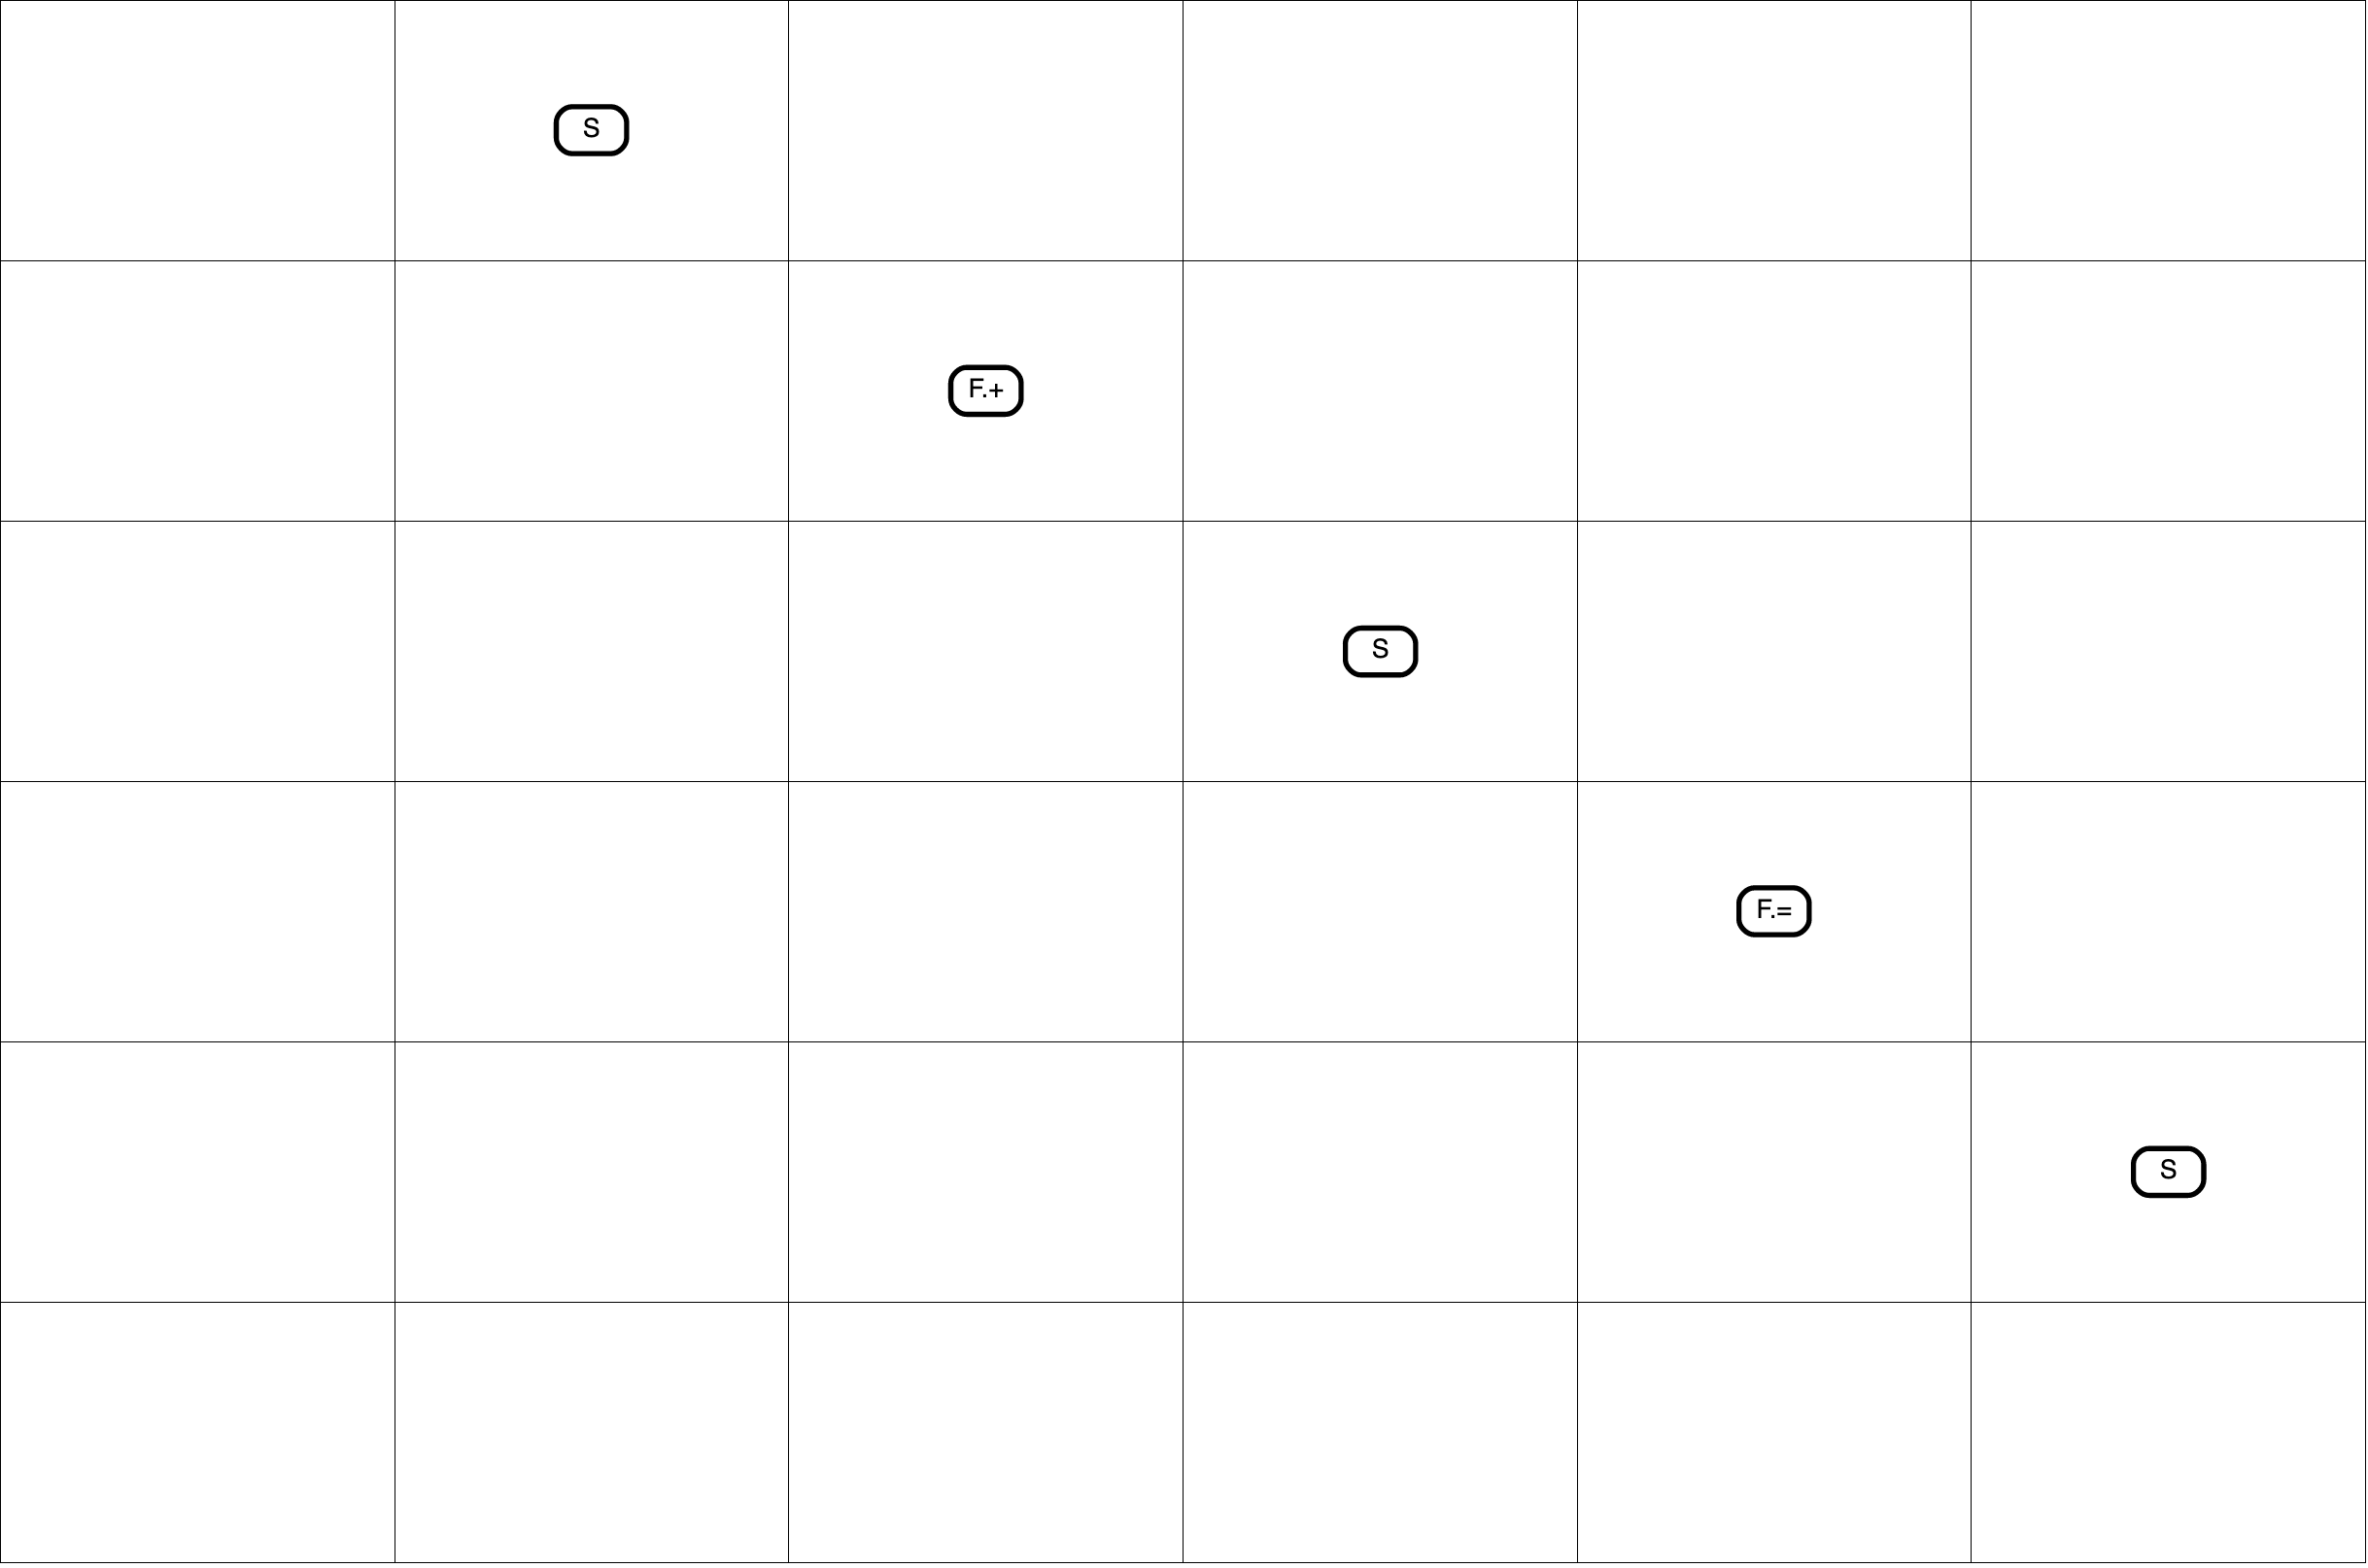
\includegraphics[width=2cm]{../figures/parse1.png}
%    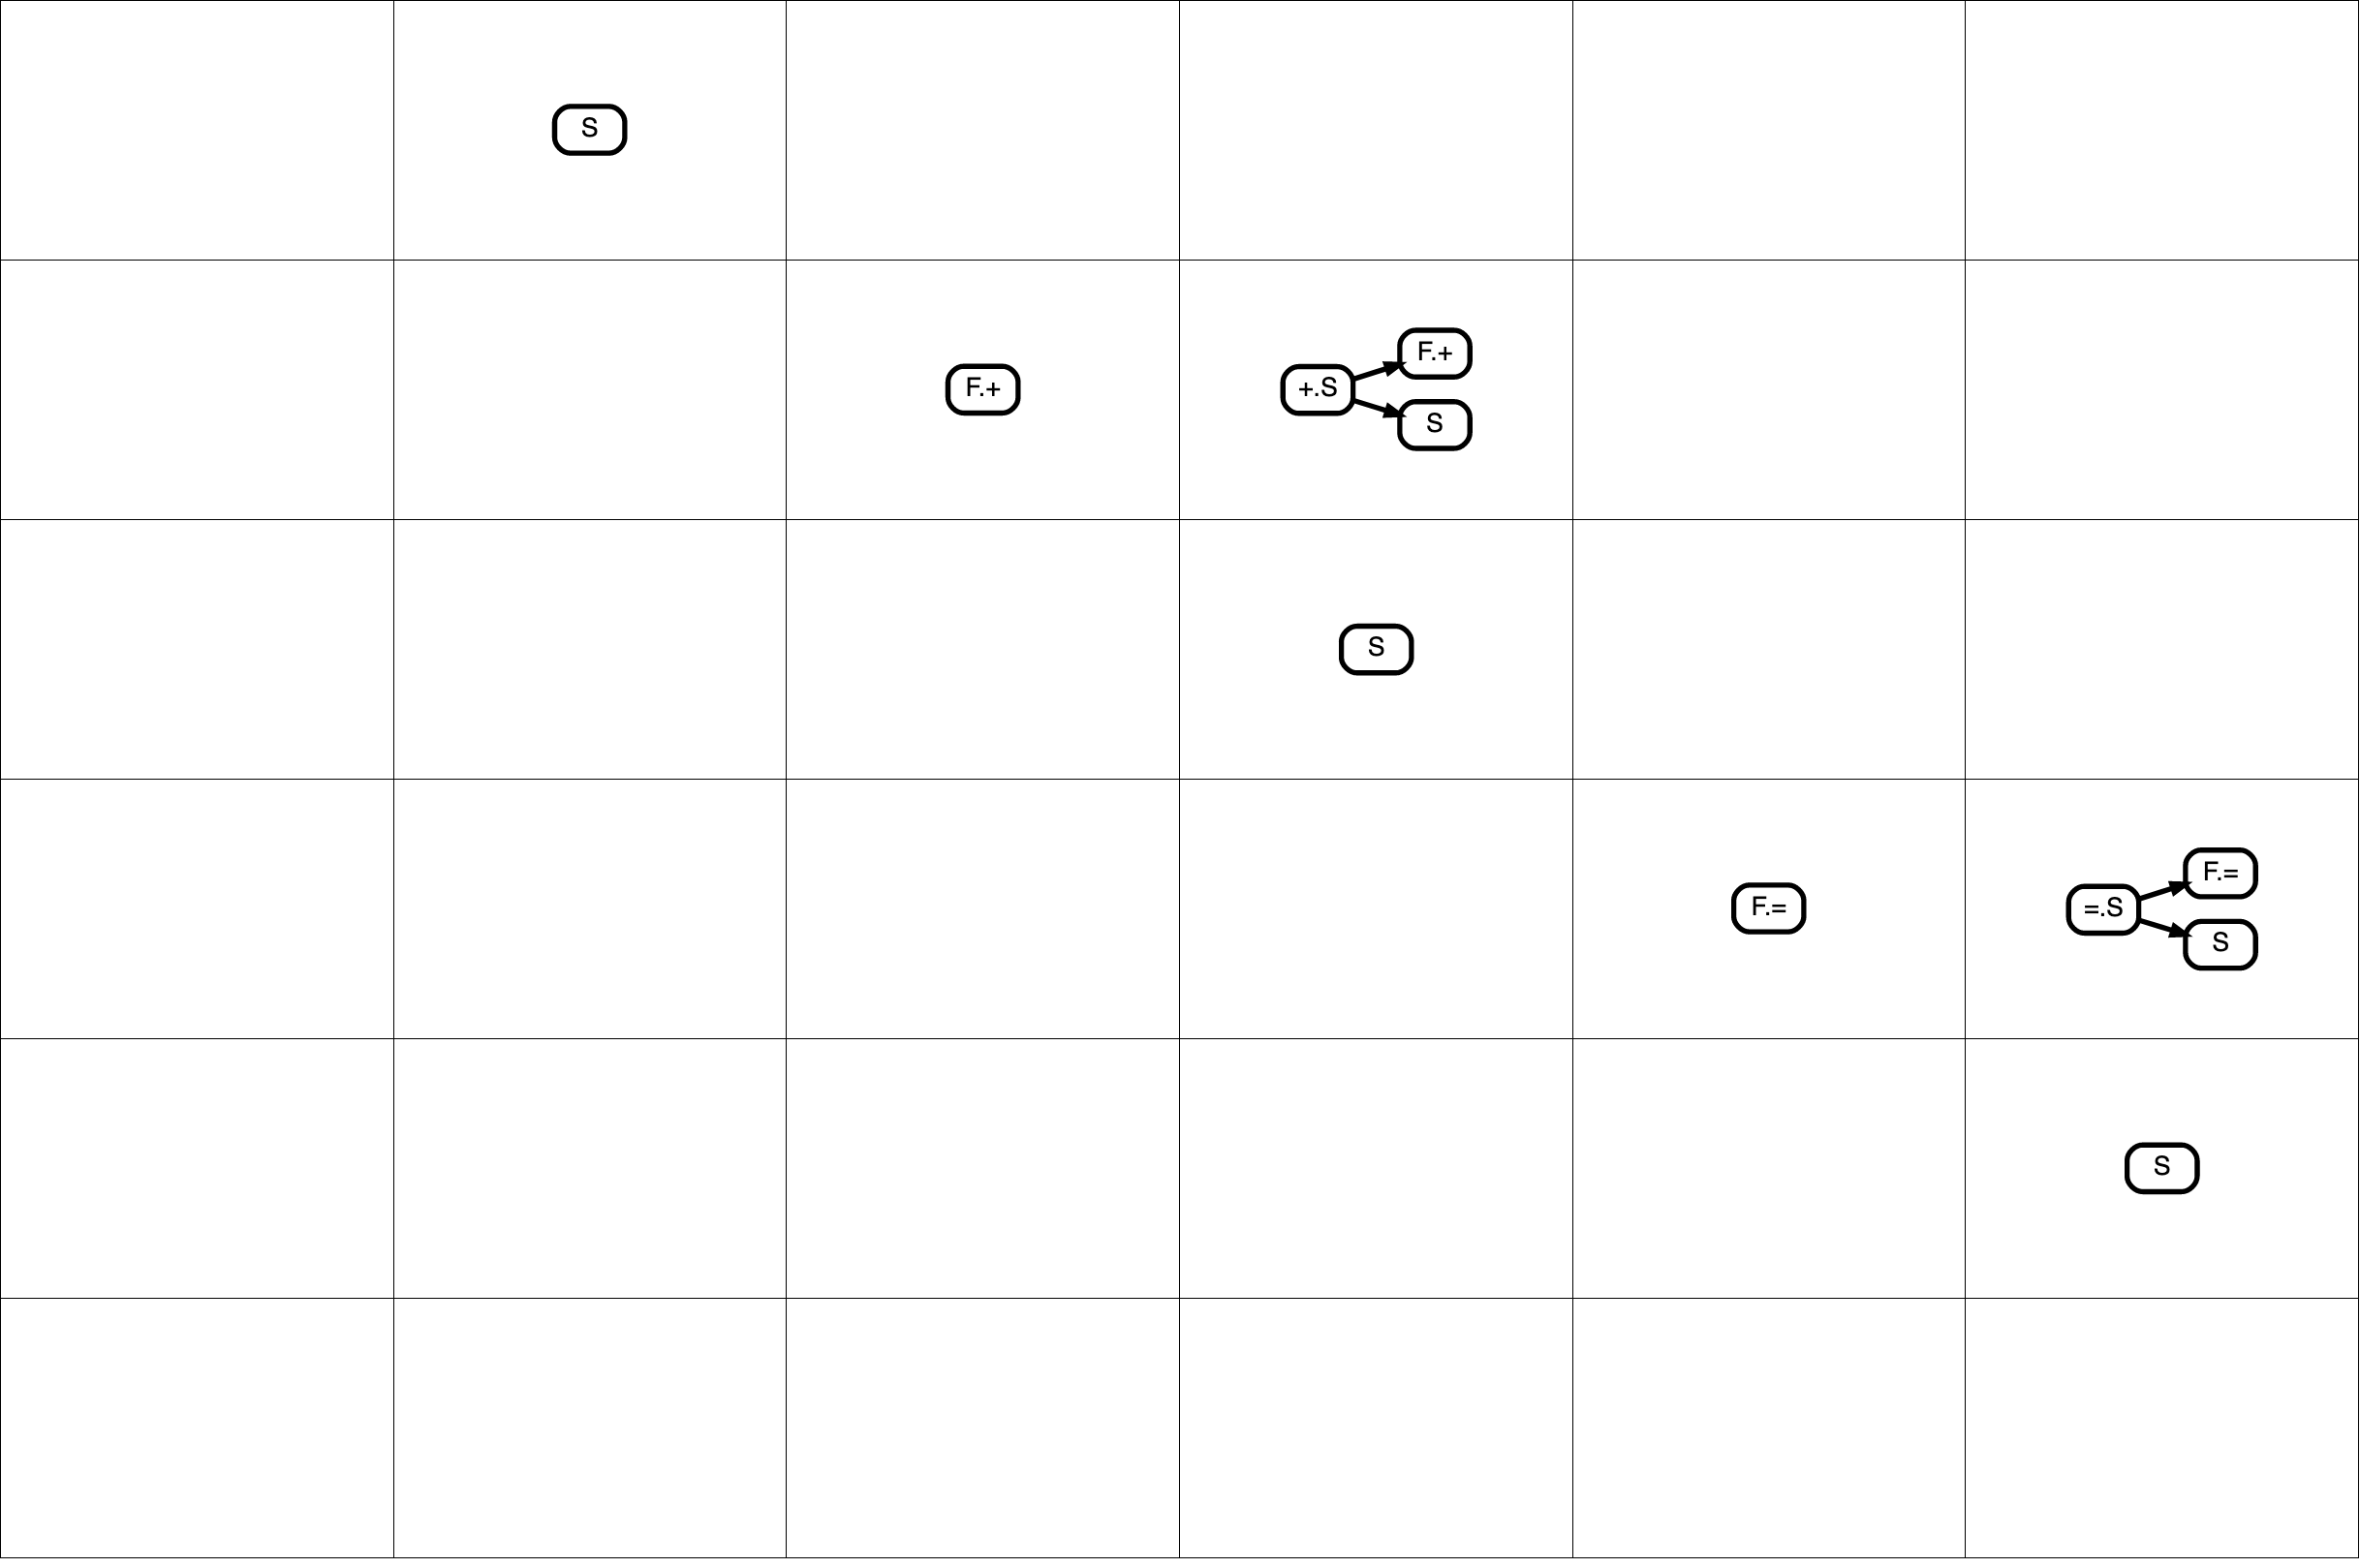
\includegraphics[width=2cm]{../figures/parse2.png}
%    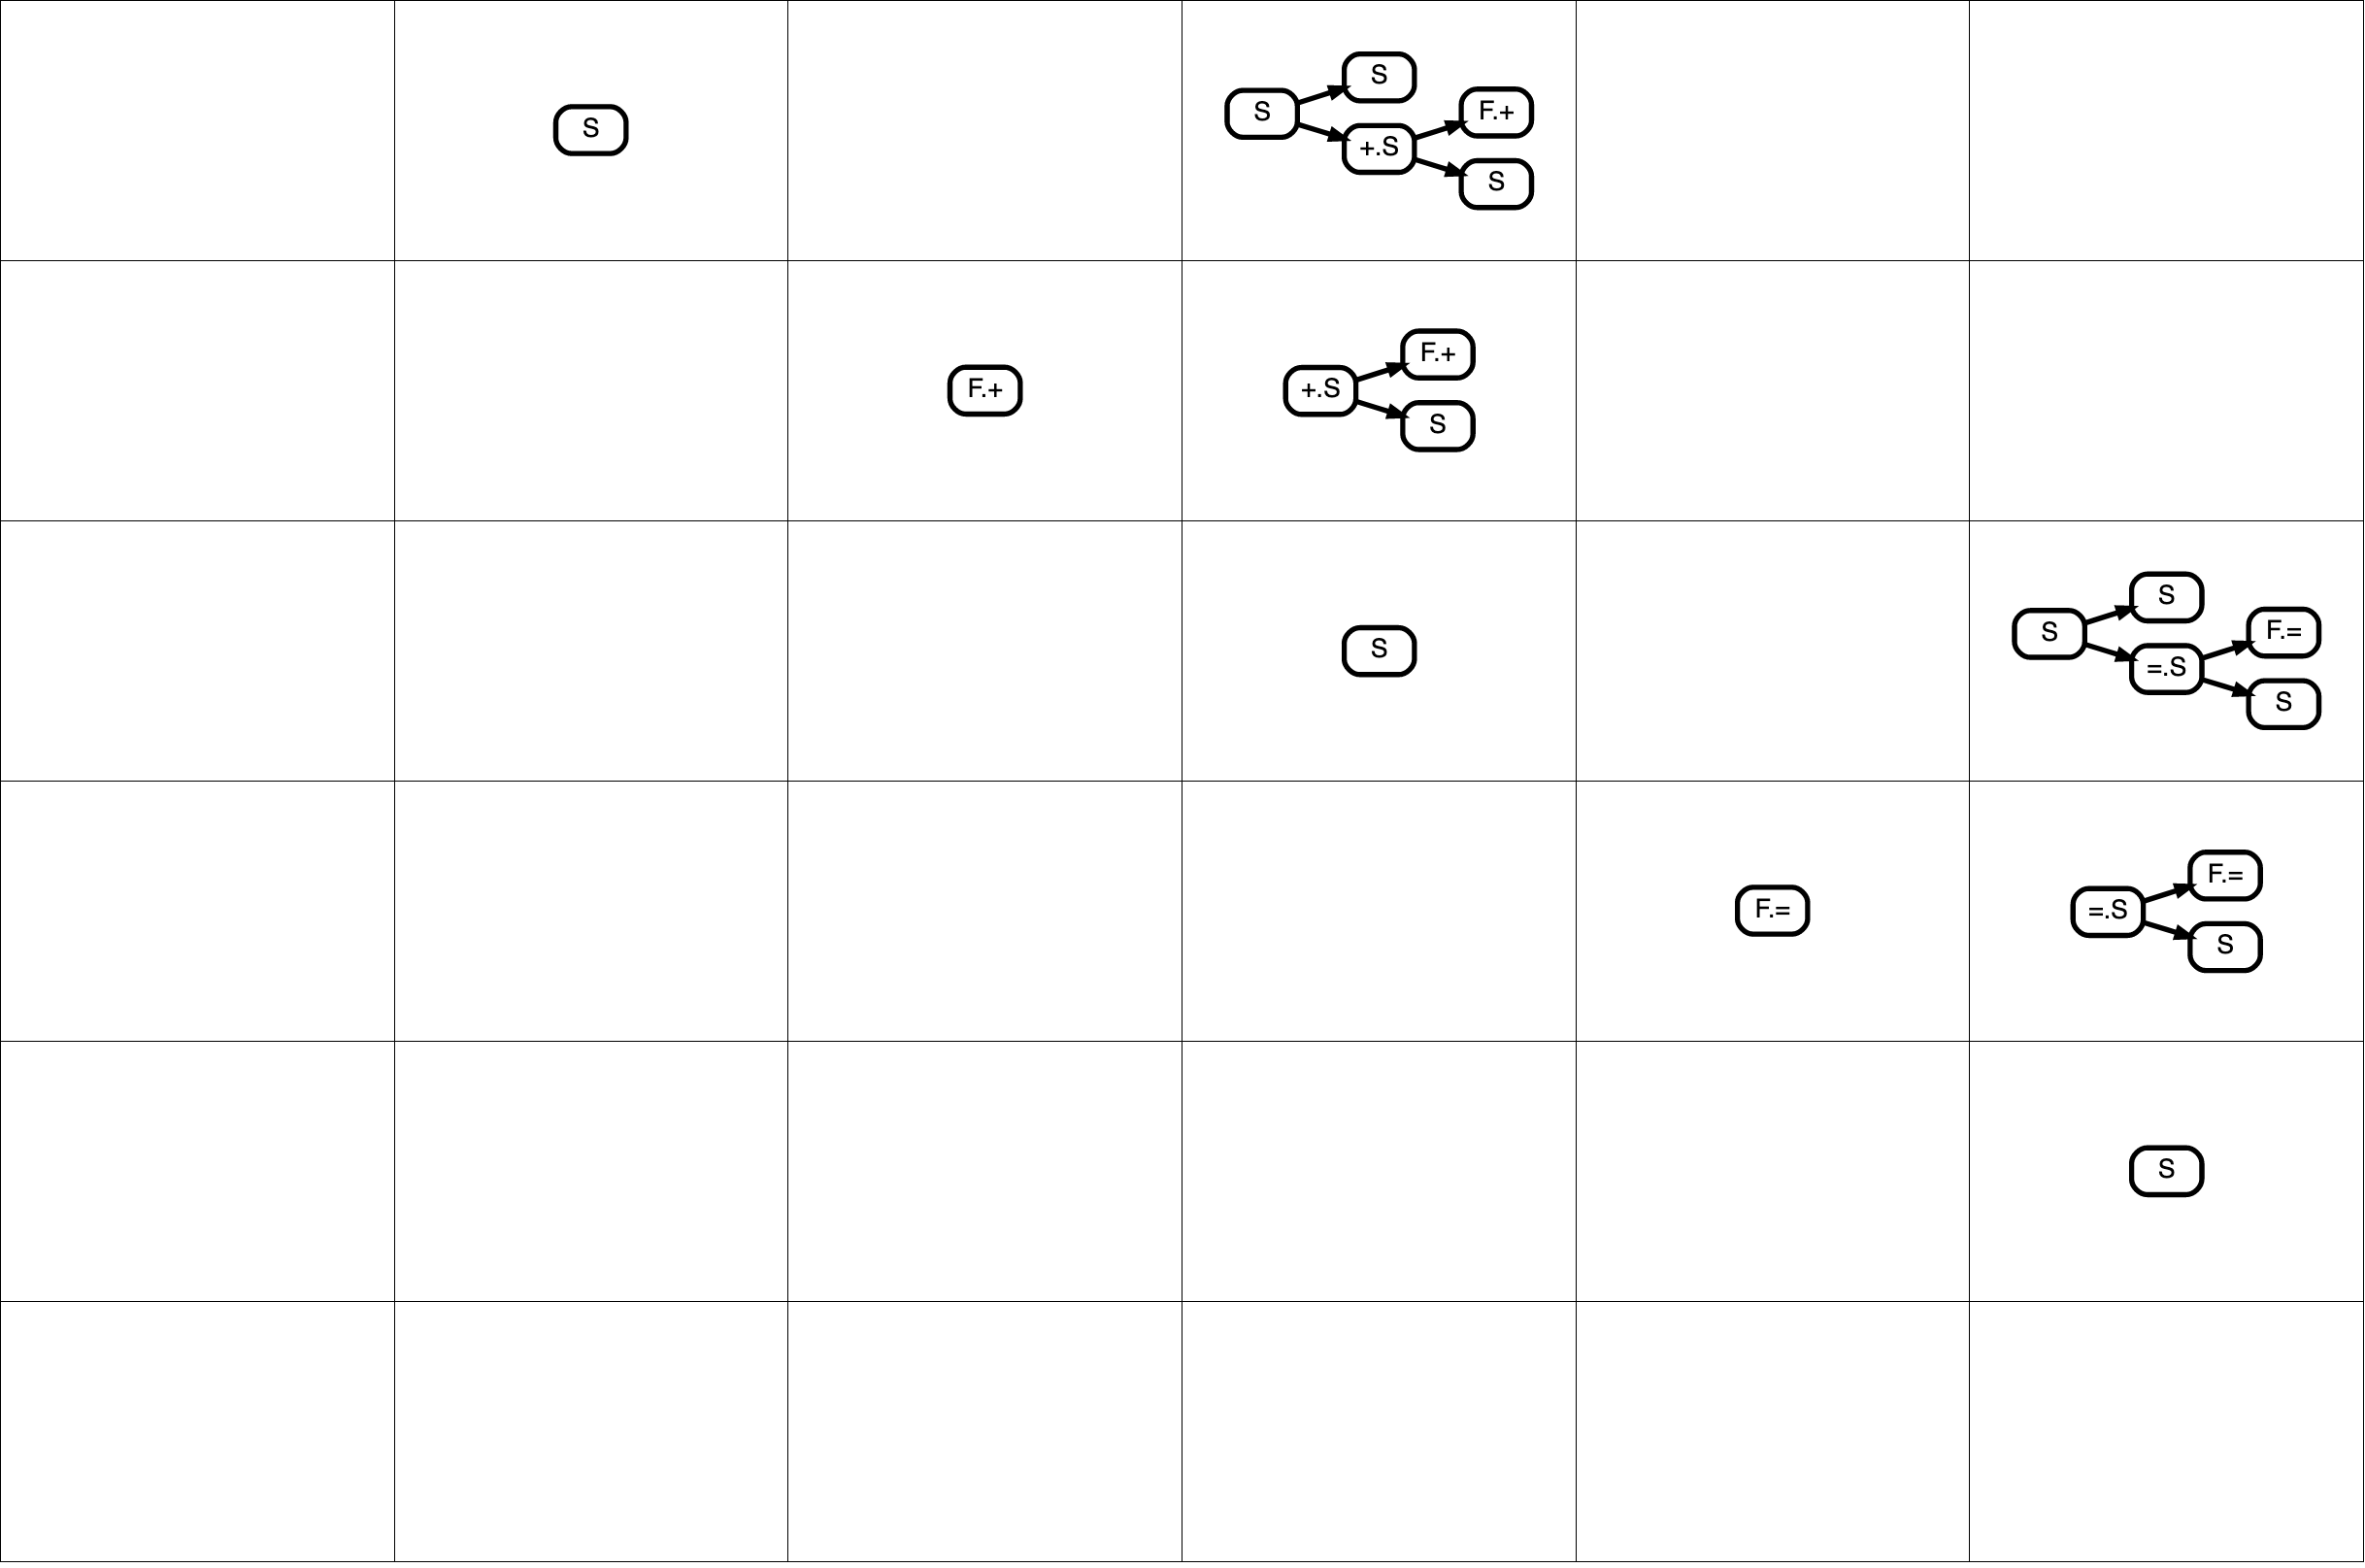
\includegraphics[width=2cm]{../figures/parse3.png}
%    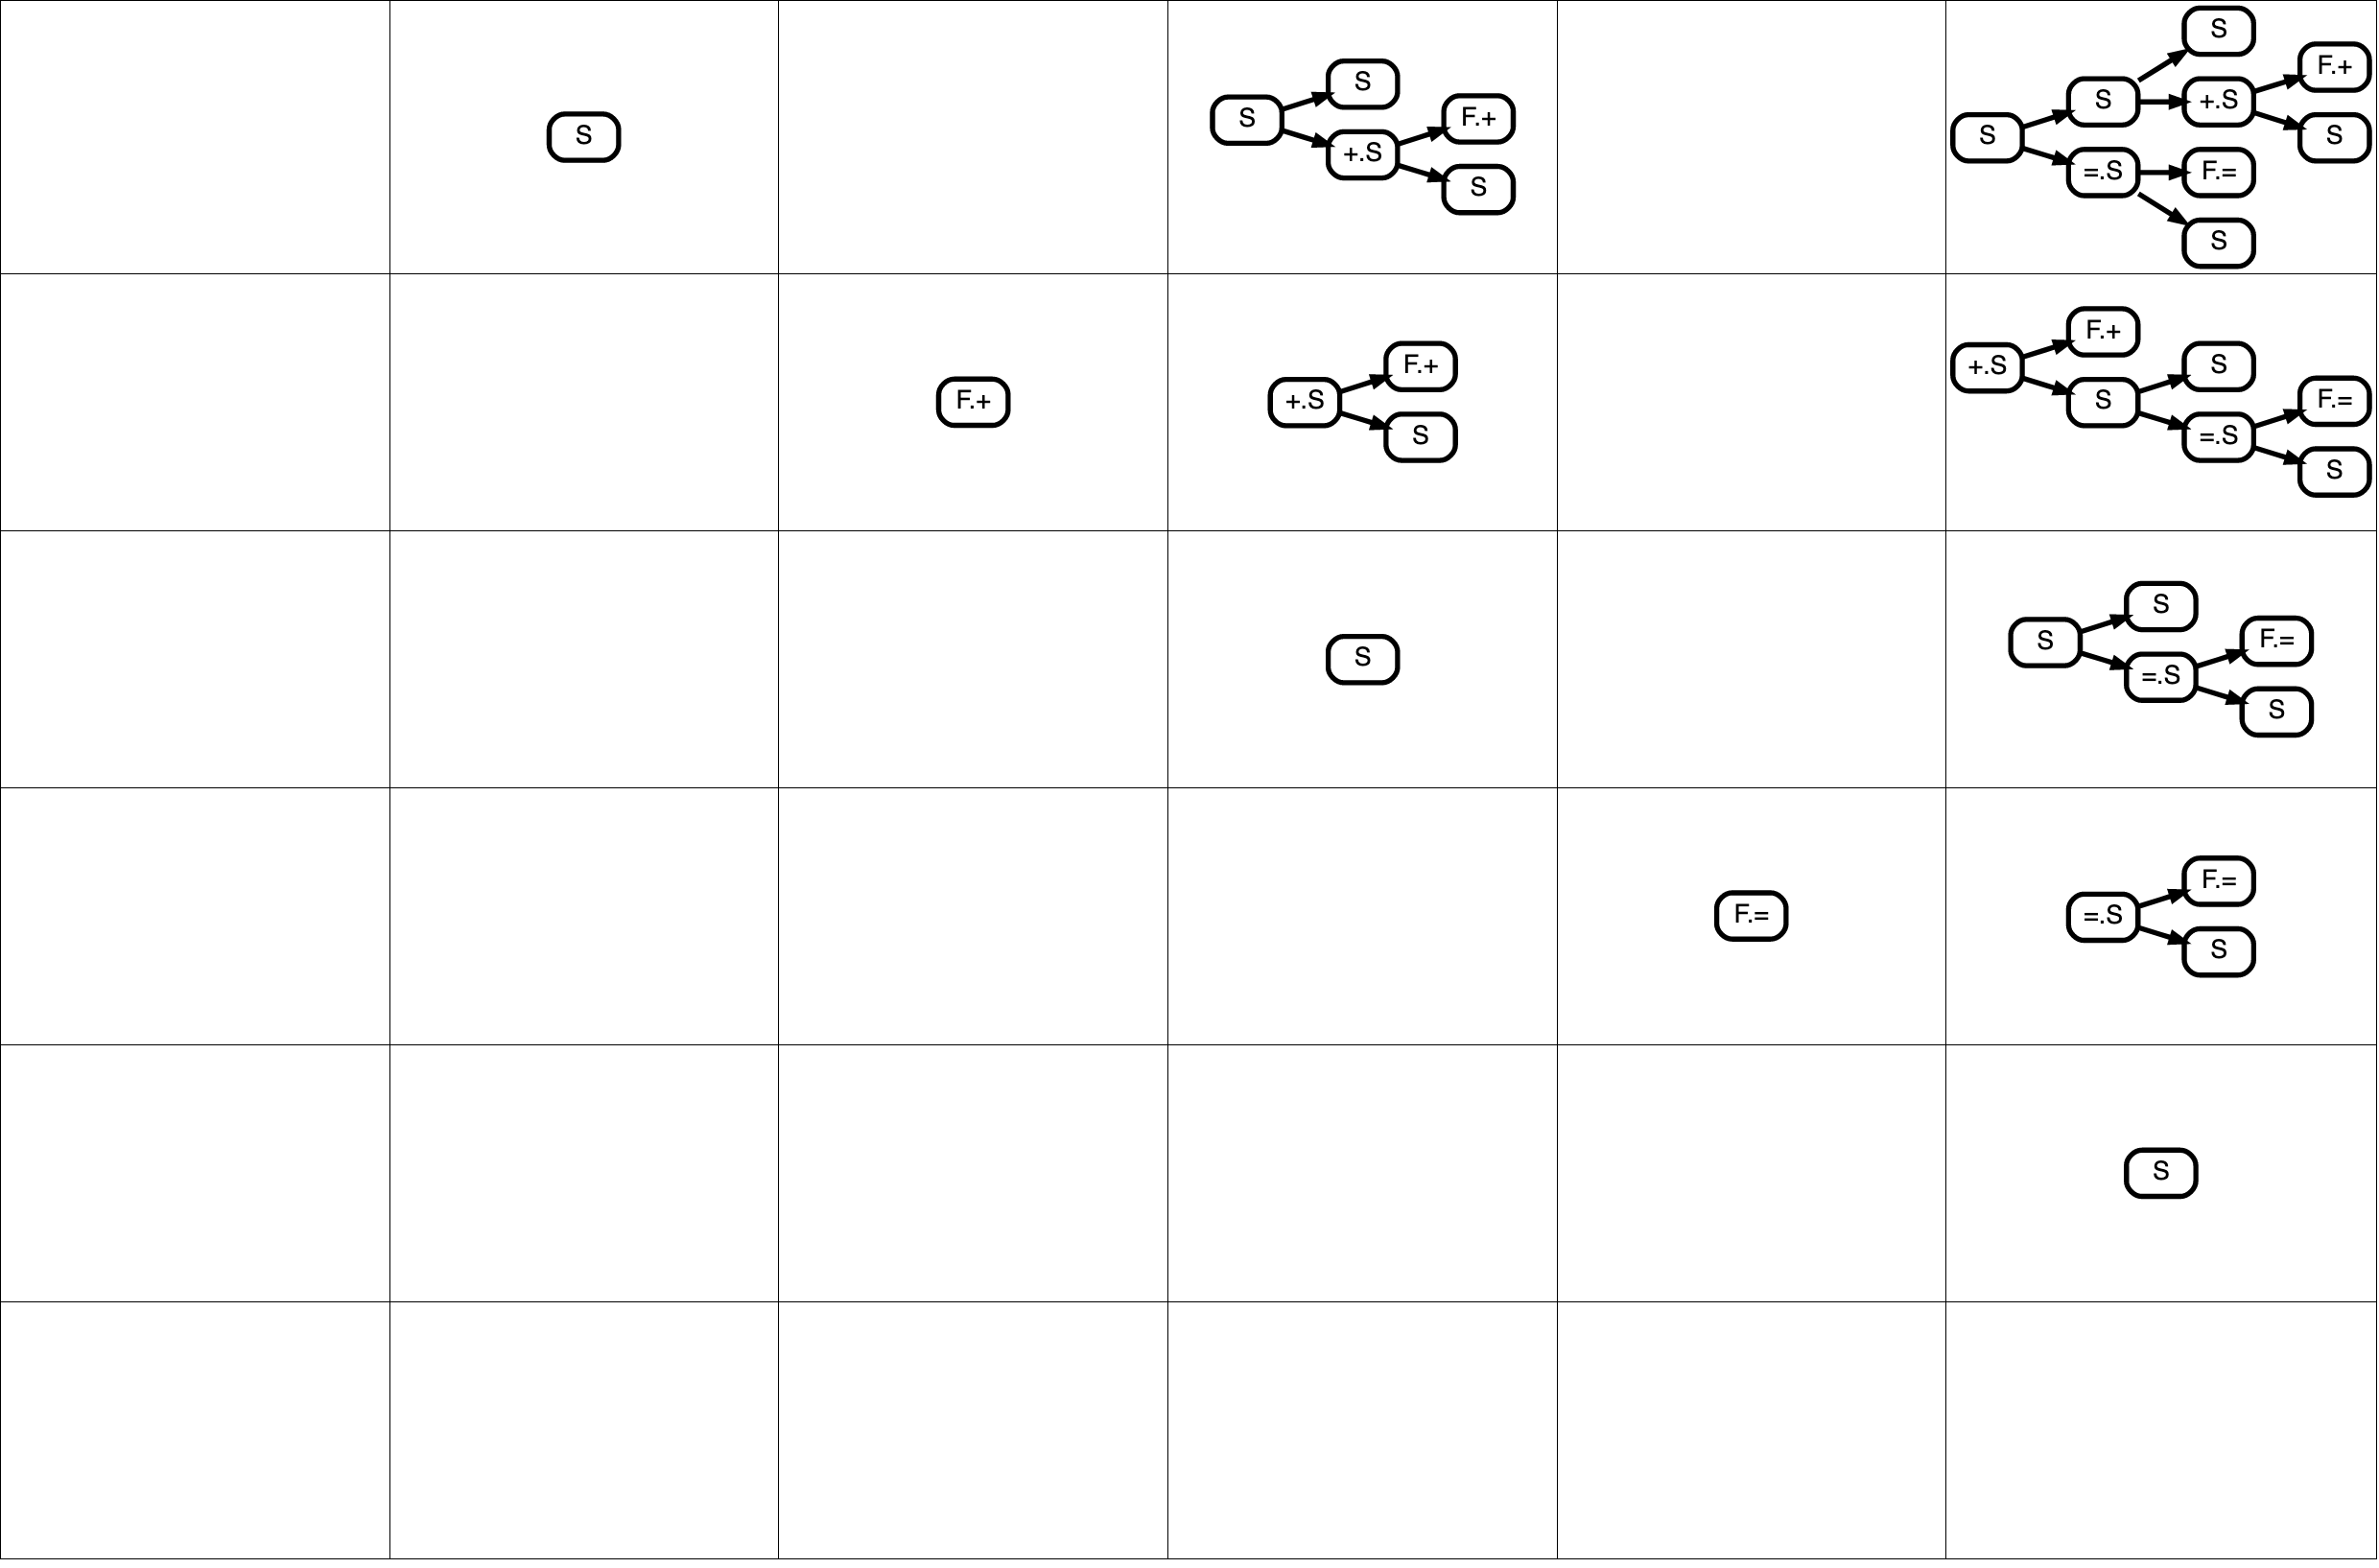
\includegraphics[width=2cm]{../figures/parse4.png}
%\end{figure}

  \begin{figure}[H]
    \[
      \mathbf{M}^* = \begin{pNiceArray}{>{\strut}ccccccc}[margin, extra-margin=2pt,colortbl-like, xdots/line-style=loosely dotted]
                       \vno & \rcr \vs{1} &  \mathcal{L}_{1,3} & \mathcal{L}_{1,3} & \rcw \mathcal{V}_{1,4} & \cdd & \mathcal{V}_{1,n} \\
                       \vdd & \ddd        &  \rcr\vs{2}        & \mathcal{L}_{2,3} & \rcw\vdd               &      & \vdd \\
                       &             &                    & \rcr\vs{3}        & \rcw                   &      & \\
                       &             &                    &                   & \mathcal{V}_{4,4}      &      & \\
                       &             &                    &                   &                        & \ddd & \\
                       &             &                    &                   &                        &      & \mathcal{V}_{n,n} \\
                       \vno & \cdd        &                    &                   &                        &      & \vno
      \end{pNiceArray}
    \]
  \end{figure}

  \noindent Depicted above is a SAT tensor representing \hlgray{$\sigma_1\:\sigma_2\:\sigma_3$}$\:\_\:\ldots\:\_$ where shaded regions demarcate known bitvector literals $\mathcal{L}_{r,c}$ (i.e., representing established nonterminal forests) and unshaded regions correspond to bitvector variables $\mathcal{V}_{r,c}$ (i.e., representing seeded nonterminal forests to be grown). Since $\mathcal{L}_{r,c}$ are fixed, we precompute them outside the SAT solver.

  \subsection{Deletion, substitution, and insertion}\label{sec:dsi}

  Deletion, substitution and insertion can be simulated by first adding a left- and right- $\varepsilon$-production to each unit production:\vspace{5pt}

  \begin{prooftree}
    \AxiomC{$\Gamma \vdash \varepsilon \in \Sigma$}
    \RightLabel{$\varepsilon\textsc{-dup}$}
    \UnaryInfC{$\Gamma \vdash (\varepsilon^+ \rightarrow \varepsilon \mid \varepsilon^+\:\varepsilon^+) \in P$}
  \end{prooftree}

  \begin{prooftree}
    \AxiomC{$\Gamma \vdash (A \rightarrow B) \in P$}
    \RightLabel{$\varepsilon^+\textsc{-int}$}
    \UnaryInfC{$\Gamma \vdash (A \rightarrow B\:\varepsilon^+ \mid \varepsilon^+\:B \mid B) \in P$}
  \end{prooftree}

  \vspace{5pt}
  \noindent To generate the sketch templates, we substitute two holes at an index-to-be-repaired, $H(\sigma, i) = \sigma_{1\ldots i-1}\:\texttt{\_ \_}\:\sigma_{i+1\ldots n}$, then invoke the SAT solver. Five outcomes are then possible:

  \begin{align}
    &\sigma_{1}\ldots\sigma_{i-1}\:\text{\hlred{$\gamma_1$}\hlred{$\gamma_2$}}\:\sigma_{i+1}\ldots\sigma_{n}, \gamma_{1, 2} = \varepsilon\label{eq:del}\\
    &\sigma_{1}\ldots \sigma_{i-1}\:\text{\hlorange{$\gamma_1$}\hlred{$\gamma_2$}}\:\sigma_{i+1}\ldots \sigma_{n}, \gamma_1 \neq \sigma_i, \gamma_2 = \varepsilon\label{eq:sub1}\\
    &\sigma_{1}\ldots \sigma_{i-1}\:\text{\hlred{$\gamma_1$}\hlorange{$\gamma_2$}}\:\sigma_{i+1}\ldots \sigma_{n}, \gamma_1 = \varepsilon, \gamma_2 \neq \sigma_i\label{eq:sub2}\\
    &\sigma_{1}\ldots\sigma_{i-1}\: \text{\hlorange{$\gamma_1$}\hlgreen{$\gamma_2$}}\:\sigma_{i+1}\ldots\sigma_{n}, \gamma_1 = \sigma_i, \gamma_2 \neq \varepsilon\label{eq:ins1}\\
    &\sigma_{1}\ldots\sigma_{i-1}\: \text{\hlgreen{$\gamma_1$}\hlorange{$\gamma_2$}}\:\sigma_{i+1}\ldots\sigma_{n}, \gamma_1 \notin \{\varepsilon, \sigma_i\}, \gamma_2 = \sigma_i\label{eq:ins2}
  \end{align}

  \noindent Eq.~(\ref{eq:del}) corresponds to deletion, Eqs.~(\ref{eq:sub1},~\ref{eq:sub2}) correspond to substitution, and Eqs.~(\ref{eq:ins1},~\ref{eq:ins2}) correspond to insertion. This procedure is repeated for all indices in the replacement set. The solutions returned by the SAT solver will be strictly equivalent to handling each edit operation as separate cases.

  \bibliography{../bib/acmart}
\end{document}